\section{Diferenças entre Abordagem Estatística Tradicional e Aprendizado Estatístico}

\begin{frame}{}
	\begin{figure}[h]
		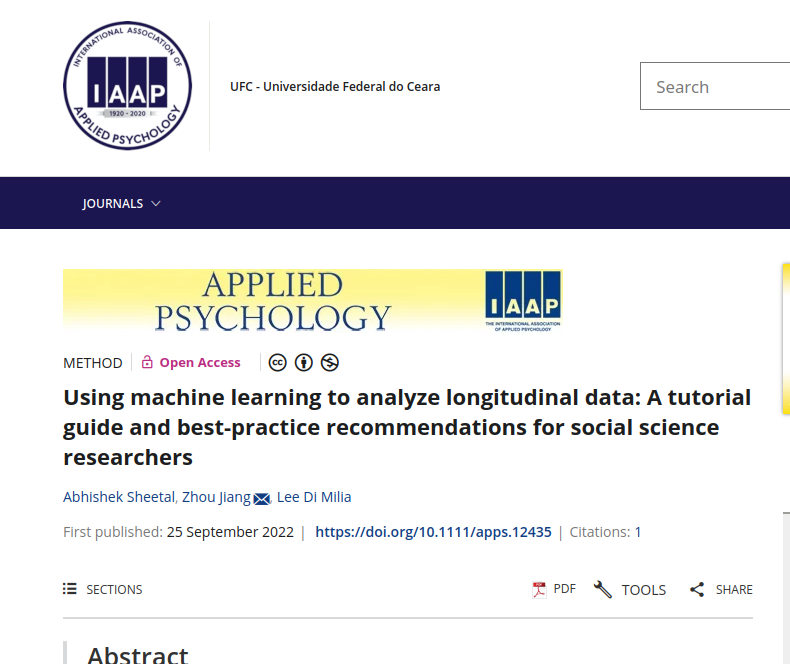
\includegraphics[scale=0.4]{imagens//secao2/artigo1.png}
	\end{figure}
\end{frame}


\begin{frame}{Possíveis complicações com abordagem Estatística Tradicional em Dados Longitudinais}
    \begin{block}{}
        \begin{itemize}
            \item Geralmente exigem técnicas mais avançadas;
            \item Herança de suposições, e.g, homoscedasticidade, normalidade, independência de observações, falta correlação entre variáveis preditoras...
        \end{itemize}
    \end{block}
\end{frame}

\begin{frame}{Suposições de alguns modelos estatísticos}
	\begin{block}{Modelos de Efeitos Fixos}
		\begin{itemize}
			\item Independência Condicional: Dados os efeitos fixos, os erros são independentes;
			\item Ausência de Correlação Serial; 
			\item O erro aleatório é não correlacionado ao longo do tempo;
			\item Homoscedasticidade dos resíduos.
		\end{itemize}
	\end{block}
\end{frame}

\begin{frame}{Suposições de alguns modelos estatísticos}
	\begin{block}{Modelos de Efeitos Aleatórios}
		\begin{itemize}
			\item Normalidade dos componentes aleatórios bem como dos resíduos;
			\item Homoscedasticidade; 
			\item Ausência de correlação serial.
		\end{itemize}
	\end{block}
\end{frame}

\begin{frame}{Suposições de alguns modelos de Aprendizado Estatísticos}
	\begin{block}{Naive Bayes}
		Independência dos preditores.
	\end{block}
	\begin{block}{Floresta Aleatória}
		Nenhum dado ausente.
	\end{block}
	\begin{block}{Redes Neurais}
		Nenhum dado ausente.
	\end{block}
	\begin{block}{Gradient Boosting}
		Nenhuma suposição inicial.
	\end{block}
\end{frame}

\begin{frame}{Comparação: Estatística Tradicional vs. Aprendizado Estatístico}
	\resizebox{\linewidth}{!}{
		\begin{tabular}{p{4cm} p{5cm} p{5cm}}
		\textbf{Atributo} & \textbf{Estatística Tradicional} & \textbf{Aprendizado de Máquina} \\
		\hline
		Adequado para & 
		Teste de hipóteses dedutivas &
		Geração de hipóteses abdutivas \\
		
		\hline 
		Forma das relações entre variáveis &
		Ajusta os dados em formas predefinidas especificadas no modelo estatístico &
		Aprende a verdadeira forma da relação entre variáveis \\
		
		\hline
		Objetivo principal &
		Testar se existem relacionamentos pré-especificados nos dados &
		Identificar padrões nos dados sem preconceitos \\
		
		\hline 
		Padrão geral de resultados &
		Baixa previsibilidade, alta explicabilidade &
		Alta previsibilidade, baixa explicabilidade \\
	\end{tabular}
	}
\end{frame}


\begin{frame}{Comparação: Estatística Tradicional vs. Aprendizado Estatístico}
	\resizebox{\linewidth}{!}{
		\begin{tabular}{p{5cm} p{4cm} p{4cm}}
			\textbf{Atributo} & \textbf{Estatística Tradicional} & \textbf{Aprendizado de 	Máquina} \\		
			\hline			
			Como confiar na análise &
			Testes de robustez &
			Modelo de teste em dados não vistos. 
			Teste a generalização por meio de análise secundária \\
			\hline
			Experiência necessária &
			Experiência em modelos estatísticos &
			Experiência em análise de diversos conjuntos de dados \\
			\hline 
			Habilidades de pesquisador &
			Treinamento em estatística &
			Treinamento em ciência de dados e programação \\

		\end{tabular}
	}
\end{frame}


\begin{frame}{Comparação: Estatística Tradicional vs. Aprendizado Estatístico}
	\resizebox{\linewidth}{!}{
	\begin{tabular}{p{3.5cm} p{4.5cm} p{4.5cm}}
		\textbf{Atributo} & \textbf{Estatística Tradicional} & \textbf{Aprendizado de Máquina} \\
		\hline 
		Poder computacional Exigido &
		Laptops modernos geralmente são suficientes &
		Requer ambiente de computação de ponta \\
		\hline
		Reutilização de modelos & 
		Precisa construir modelos diferentes para cada objetivo &
		Um algoritmo pode ser reutilizado para diferentes objetivos \\
		\hline
		Número de preditores &
		Limitado pela correlação entre variáveis &
		Limitado pelo poder computacional \\
	\end{tabular}}
\end{frame}













